\section{\label{section:computational approach}Computational Approach}

\begin{figure}
  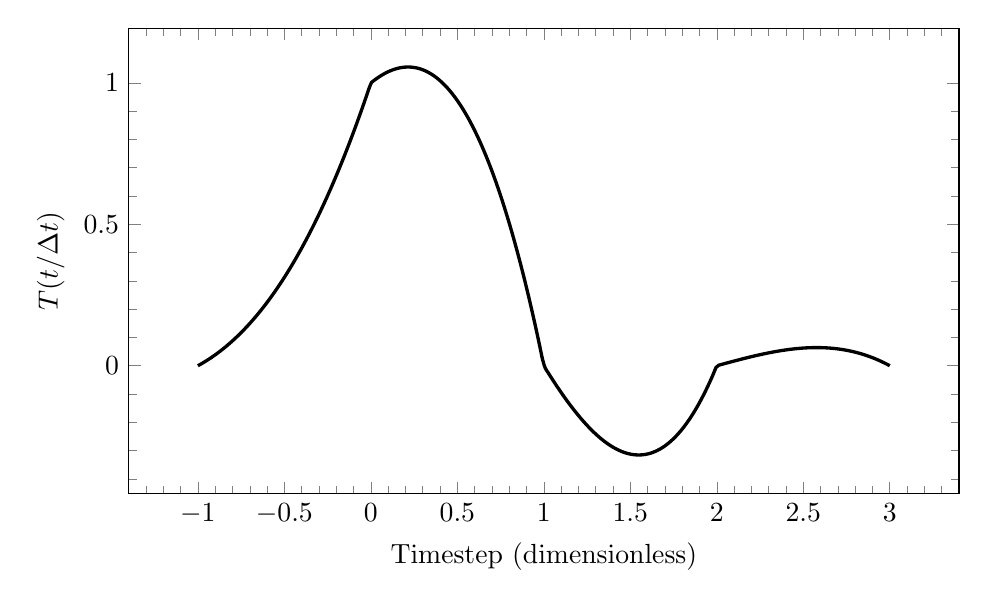
\begin{tikzpicture}[
  declare function = {
    basis(\x) = 
      and(-1 <= \x, \x < 0)*(1+x)*(2+x)*(3+x)/6 +
      and(0  <= \x, \x < 1)*(1-x)*(1+x)*(2+x)/2 +
      and(1  <= \x, \x < 2)*(1-x)*(2-x)*(1+x)/2 + 
      and(2  <= \x, \x < 3)*(1-x)*(2-x)*(3-x)/6 + 
      or(\x <-1, \x > 3)*0;
  }
  ]

  \begin{axis}[width=\columnwidth, height=0.61803398875\columnwidth,
      %xtick={-4, -3, -2, -1},
      minor x tick num={4},
      minor y tick num={4},
      xlabel = Timestep (dimensionless),
      ylabel = {$T(t/\Delta t)$}
      %xticklabels={$-4\Delta t$, $-3\Delta t$, $-2\Delta t$, $-\Delta t$}
  ]
  
  \addplot[very thick, domain=-1:3, smooth, samples=256] {basis(x)};
  \end{axis}
\end{tikzpicture}

  \caption{\label{fig:interpolation basis} Nonorthogonal and $C^0$-continuous temporal basis function $T(t)$ constructed from intervals of fourth-order Lagrange polynomials.}
\end{figure}
To solve \cref{eq:rotating liouville,eq:radiated envelope} for each of $N_s$ \qds{} at $N_t$ equally-spaced timesteps, we begin with a suitable representation of $\tilde{\vb{P}}(\vb{r}, t)$ in terms of spatial and temporal basis functions, i.e.~
\begin{equation}
  \tilde{\vb{P}}(\vb{r}, t) = \sum_{\ell=0}^{N_s - 1} \sum_{m = 0}^{N_t - 1} \tilde{\alpha}_{\ell m} \vb{S}_\ell(\vb{r}) T(t - m \, \Delta t).
  \label{eq:basis function representation}
\end{equation}
As the wavelength of any radiation in the system far exceeds the dimensions of the \qds{} under consideration, we take $\vb{S}_\ell(\vb{r}) \equiv \vb{d}_\ell \delta(\vb{r} - \vb{r}_\ell)$.
Such a discretization additionally discretizes \cref{eq:rotating liouville}, forming a set of $N_s$ first-order differential equations coupled through radiative processes with retardation.
Furthermore, we require the $T(t)$ to have finite support as well as causal and interpolatory properties so as to recover $\tilde{\vb{P}}$, $\partial_t \tilde{\vb{P}}$, and $\partial^2_t \tilde{\vb{P}}$ at every timestep.
Accordingly, we have elected to use a set of backwards-looking Lagrange polynomials of order $\ge 4$, forming a temporal basis set with functions similar to the one shown in \cref{fig:interpolation basis}.
These functions  reliably interpolate smooth functions with controllable error and have a long history of use in studies of electromagnetic systems~\textcolor{red}{\cite{SHANKER,SHANKER,SHANKER}}.

Combining \cref{eq:radiated envelope,eq:basis function representation} and projecting the resulting field onto the $\vb{S}_\ell$ and $T_m$ basis functions produces a marching-on-in-time system of the form
\begin{equation}
  \mathcal{L}^{(k)} + \sum_{m = 0}^{k} \mathcal{Z}^{(m)} \mathcal{A}^{(k - m)} = \mathcal{F}^{(k)}.
  \label{eq:zmatrix}
\end{equation}
In this (block $N_s \times N_s$) matrix equation, $\mathcal{A}^{(k)}$ denotes the (spatial) collection of $\tilde{\alpha}_{\ell k}$ and
\begin{subequations}
  \begin{align}
    \mathcal{L}^{(m)}_{\ell} &= \big\langle \mathbf{S}_\ell(\vb{r}), \tilde{\vb{E}}_L(\vb{r}, m \, \Delta t) \big\rangle \\
    \mathcal{Z}^{(m)}_{\ell \ell'} &= \big\langle \mathbf{S}_\ell(\vb{r}), \tilde{\mathfrak{F}}\{ \mathbf{S}_{\ell'}(\mathbf{r}) T(m \, \Delta t) \} \big\rangle \\
    \mathcal{F}^{(m)}_\ell &= \big\langle \mathbf{S}_\ell(\vb{r}), \tilde{\mathbf{E}}(\vb{r}, m \, \Delta t) \big\rangle.
  \end{align}
  \label{eq:projections}
\end{subequations}
with $\langle \cdot, \cdot \rangle$ representing a projection operation.
As we have elected to use a uniform $\Delta t$, $\mathcal{Z}$ represents a block Toeplitz and lower triangular space/time matrix and \cref{eq:zmatrix} provides a means of calculating $\mathcal{F}^{(m)}$ given only $\mathcal{A}^{(m' \le m)}$.

To link $\mathcal{A}^{(m)}$ with the density matrix in \cref{eq:rotating liouville}, we take
\begin{equation}
  \tilde{\alpha}_{\ell m} \equiv \tilde{\rho}_{\ell, 01}(t = m \, \Delta t)
  \label{eq:polarization definition}
\end{equation}
as the off-diagonal matrix elements (coherences) of $\tilde{\rho}_{\ell}$ directly characterize the dipole radiating at $\vb{r}_\ell$ under the rotating-wave approximation.
Consequently, determining $\mathcal{A}^{(m + 1)}$ amounts to integrating \cref{eq:rotating liouville} from $t = m \, \Delta t$ to $t = \qty(m + 1) \, \Delta t$ for every \qd{} in the system.
For this, we make use of the predictor/corrector scheme detailed in~\cite{Glaser2009}.
Defining $t_m \equiv m \, \Delta t$ and approximating $\tilde{\rho}(t)$ as a weighted sum of complex exponentials, the predictor/corrector scheme proceeds with an extrapolation predictor step,
\begin{equation}
  \tilde{\rho}_\ell(t_{m + 1}) \leftarrow \sum_{w = 0}^{W-1} \mathcal{P}_w^{\qty(0)} \tilde{\rho}_\ell(t_{m-w}) + \mathcal{P}_w^{\qty(1)} \, \partial_t \tilde{\rho}_\ell(t_{m-w}),
  \label{eq:predictor}
\end{equation}
and iterated corrector steps,
\begin{equation}
  \begin{aligned}
    \tilde{\rho}_\ell(t_{m + 1}) &\leftarrow \mathcal{C}_{m+1}^{\qty(1)} \, \partial_t \tilde{\rho}_\ell(t_{m+1}) \\
                                 &+ \sum_{w = 0}^{W - 1} \mathcal{C}_w^{\qty(0)} \tilde{\rho}_\ell(t_{m-w}) + \mathcal{C}_w^{\qty(1)} \, \partial_t \tilde{\rho}_\ell(t_{m-w}).
  \end{aligned}
  \label{eq:corrector}
\end{equation}
We precompute $\mathcal{P}_w^{\qty(0, 1)}$ and $\mathcal{C}_w^{\qty(0, 1)}$ coefficients with a least-squares procedure based on spectral and error considerations given in~\cite{Glaser2009}.
\textcolor{red}{These coefficients play the same role as $1/3$ and $1/6$ in a standard fourth-order Runge-Kutta implementation.}

To summarize, one timestep of our solution strategy proceeds as follows:
\begin{enumerate}
  \item At timestep $m$, use \cref{eq:predictor,eq:polarization definition} to predict $\mathcal{A}^{(m + 1)}$.
    This prediction depends only on the known history of the system and does not require the calculation of any electromagnetic interactions.
  \item Use \cref{eq:zmatrix} to calculate $\mathcal{F}^{(m + 1)}$.
    Having approximated $\mathcal{A}^{(m + 1)}$ in step 1, $\mathcal{F}^{(m + 1)}$ will contain information from \qds{} within $c \, \Delta t$ of each other.
  \item Produce $\partial_t \tilde{\rho}(t_{m + 1})$ (and thus $\partial_t \mathcal{A}^{(m + 1)}$) by evaluating \cref{eq:rotating liouville} with the $\mathcal{F}^{(m+1)}$ found in step 2.
  \item Correct $\mathcal{A}^{(m + 1)}$ with \cref{eq:corrector} and $\partial_t \mathcal{A}^{(m + 1)}$ found in step 3.
    Repeat steps 2 through 4 until $\mathcal{A}^{(m + 1)}$ has sufficiently converged, then set $m \leftarrow m + 1$.
\end{enumerate}
